\documentclass[tikz,border=2pt]{standalone}
\usepackage{amsmath}
\usepackage{pgfplots}
\pgfplotsset{compat=1.18}
\usetikzlibrary{arrows.meta}
\begin{document}
% For l = list(1, 2, 3): l[1] is a list containing the first element (box kept),
% l[[1]] is the element itself, the number 1 (box removed).
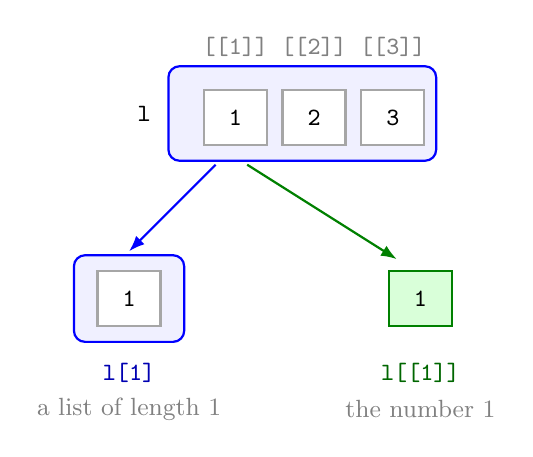
\begin{tikzpicture}[font=\small, >={Latex[length=2mm]},
  cell/.style={draw, thick, gray!70, fill=white, minimum width=8mm, minimum height=7mm, inner sep=0pt, font=\small\ttfamily, text=black}]
  % the list l
  \draw[blue, thick, rounded corners=4pt, fill=blue!6] (2.0,2.4) rectangle (5.4,3.6);
  \node[anchor=east, font=\small\ttfamily] at (1.9,3.0) {l};
  \foreach \v [count=\i] in {1,2,3} {
    \node[cell] at (1.85+1.0*\i,2.95) {\v};
    \node[gray, font=\small\ttfamily] at (1.85+1.0*\i,3.85) {[[\i]]};
  }
  % l[1]
  \draw[->, thick, blue] (2.6,2.35) -- (1.5,1.25);
  \draw[blue, thick, rounded corners=4pt, fill=blue!6] (0.8,0.1) rectangle (2.2,1.2);
  \node[cell] at (1.5,0.65) {1};
  \node[font=\small\ttfamily, blue!70!black] at (1.5,-0.3) {l[1]};
  \node[gray] at (1.5,-0.75) {a list of length 1};
  % l[[1]]
  \draw[->, thick, green!50!black] (3.0,2.35) -- (4.9,1.15);
  \node[cell, draw=green!50!black, fill=green!15] at (5.2,0.65) {1};
  \node[font=\small\ttfamily, green!40!black] at (5.2,-0.3) {l[[1]]};
  \node[gray] at (5.2,-0.75) {the number 1};
\end{tikzpicture}
\end{document}
